% -------------------------------------------------------------------------------
% Establish page structure & font.
\documentclass[12pt]{report}

\usepackage[total={6.5in, 9in},
	left=1in,
	right=1in,
	top=1in,
	bottom=1in,]{geometry} % Page structure

\usepackage{graphicx} % Required for inserting images
\graphicspath{{../../.images}} % Any additional images I use (BCU logo, etc) are from here.

\usepackage[utf8]{inputenc} % UTF-8 encoding
\usepackage[T1]{fontenc} % T1 font
\usepackage{float}  % Allows for floats to be positioned using [H], which correctly
                    % positions them relative to their location within my LaTeX code.
\usepackage{subcaption}
\usepackage{csquotes}

% -------------------------------------------------------------------------------
% Declare biblatex with custom Harvard BCU styling for referencing.
\usepackage[
    useprefix=true,
    maxcitenames=3,
    maxbibnames=99,
    style=authoryear,
    dashed=false, 
    natbib=true,
    url=false,
    backend=biber
]{biblatex}

\usepackage[british]{babel}

% Additional styling options to ensure Harvard referencing format.
\renewbibmacro*{volume+number+eid}{
    \printfield{volume}
    \setunit*{\addnbspace}
    \printfield{number}
    \setunit{\addcomma\space}
    \printfield{eid}}
\DeclareFieldFormat[article]{number}{\mkbibparens{#1}}

\addbibresource{Proposal.bib}

% -------------------------------------------------------------------------------
% To prevent "Chapter N" display for each chapter
\usepackage[compact]{titlesec}
\usepackage{wasysym}
\usepackage{import}

\titlespacing*{\chapter}{0pt}{-2cm}{0.5cm}
\titleformat{\chapter}[display]
{\normalfont\bfseries}{}{0pt}{\Huge}

% -------------------------------------------------------------------------------
% Custom macro to make an un-numbered footnote.

\newcommand\blfootnote[1]{
    \begingroup
    \renewcommand\thefootnote{}\footnote{#1}
    \addtocounter{footnote}{-1}
    \endgroup
}

% -------------------------------------------------------------------------------
% Fancy headers; used to show my name, BCU logo and current chapter for the page.
\usepackage{fancyhdr}
\usepackage{calc}
\pagestyle{fancy}

\setlength\headheight{37pt} % Set custom header height to fit the image.

\renewcommand{\chaptermark}[1]{%
    \markboth{#1}{}} % Include chapter name.


% Lewis Higgins - ID 22133848           [BCU LOGO]                [CHAPTER NAME]
\lhead{Lewis Higgins - ID 22133848~~~~~~~~~~~~~~~
\includegraphics[width=1.75cm]{BCU}}
\fancyhead[R]{\leftmark}

% ------------------------------------------------------------------------------
% Used to add PDF hyperlinks for figures and the contents page.

\usepackage{hyperref}

\hypersetup{
    colorlinks=true,
    linkcolor=black,
    filecolor=magenta,
    urlcolor=blue,
    citecolor=black,
}

% ------------------------------------------------------------------------------
\usepackage{xcolor} 
\usepackage{colortbl}
\usepackage{longtable}
\usepackage{amssymb}
% ------------------------------------------------------------------------------
\usepackage{tcolorbox}
\newcommand{\para}{\vspace{7pt}\noindent}
% -------------------------------------------------------------------------------

\title{Leveraging Convolutional Neural Networks for the identification of Pneumonia}
\author{Lewis Higgins - Student ID 22133848}
\date{March 2025}

% -------------------------------------------------------------------------------

\begin{document}


\makeatletter
\begin{titlepage}
    \begin{center}
        
\includegraphics[width=0.7\linewidth]{BCU}\\[4ex]
        {\huge \bfseries \@title}\\[2ex]
        {\large \bfseries  Project Proposal}\\[50ex]
        {\@author}\\[2ex]
        {CMP6228 - Deep Neural Networks}\\[2ex]
        {Module Coordinator: Khalid Ismail}\\[2ex]
        {Word count excluding figures, references and appendices: XXXX / 1500}\\[10ex]
    \end{center}
\end{titlepage}
\makeatother
\thispagestyle{empty}
\newpage

% Page counter trick so that the contents page doesn't increment it.
\setcounter{page}{0}

\tableofcontents
\thispagestyle{empty}

\chapter*{Introduction}
\addcontentsline{toc}{chapter}{Introduction}

In this report, a novel solution is proposed to address a significant data science problem in the medical field, in the form of 
a deep neural network to accurately identify the presence of pneumonia from an image of a chest X-ray. To do so, this neural network 
will be trained on a publicly available dataset that has been previously seen across many publications, and advanced techniques 
for the model will be discussed.

\para This proposal will specifically cover the motivation behind this project before exploring related literature and previous works 
in great depth. To conclude, an optimal model will be proposed based on the knowledge extracted from these related works. 

% ! Weak. Come back to this probably at the very end.


\chapter{Motivation and objectives}

\section{Subject area}

Pneumonia is a lower respiratory tract infection (LRTI) commonly caused by viruses or bacteria wherein the alveoli of the lungs 
become clogged with pus and fluid, which can be life-threatening in people of any age, but especially in children and the elderly
\autocite{nhsPneumonia2017}. The World Health Organisation (WHO) state that pneumonia is the single largest infectious cause of death 
in children, killing 808,000 children under the age of 5 in 2017 \autocite{whoPneumonia}. Furthermore, even if pneumonia is survived during the initial 
infection, \textcite{allinsonEarlyChildhoodLower2023} studied that those who contract the condition as a child are 93\% more likely to die from 
respiratory diseases later in life than those who did not.

\para It is therefore imperative that recent technological advancements are leveraged for the quick diagnosis of the infection to allow swift 
treatment to avoid life-threatening consequences, both in the short-term and long-term. 

\section{Dataset choice}
The chosen dataset is sourced from the Mendeley data repository \autocite{mendeleydataLargeDatasetLabeled}, uploaded and created by  
\textcite[p.1127]{kermanyIdentifyingMedicalDiagnoses2018} in their research of the applications of neural networks for medical diagnoses.
The dataset contains 5,856 images of chest X-ray scans of children taken from the
Guangzhou Women and Children's Medical Center in China, and is 1.18GB in size. \textcite[p.e1]{kermanyIdentifyingMedicalDiagnoses2018} 
state that the data was heavily screened and scrutinized for confirmation before labelling, which was done by removing low quality or unreadable images,
and then consulting two expert physicians before labelling the images. The physicians' labelled set was then presented to a third expert, 
who confirmed their validity. Because of this, there is absolute certainty in the authenticity and validity of the data itself as well as its 
ground truth labels.
There are only two classes of images: those with 
pneumonia and those without, as depicted by Figures \ref{fig:SampleNORMAL} and \ref{fig:SamplePNEUMONIA}.

\begin{figure}[H]
    \centering
    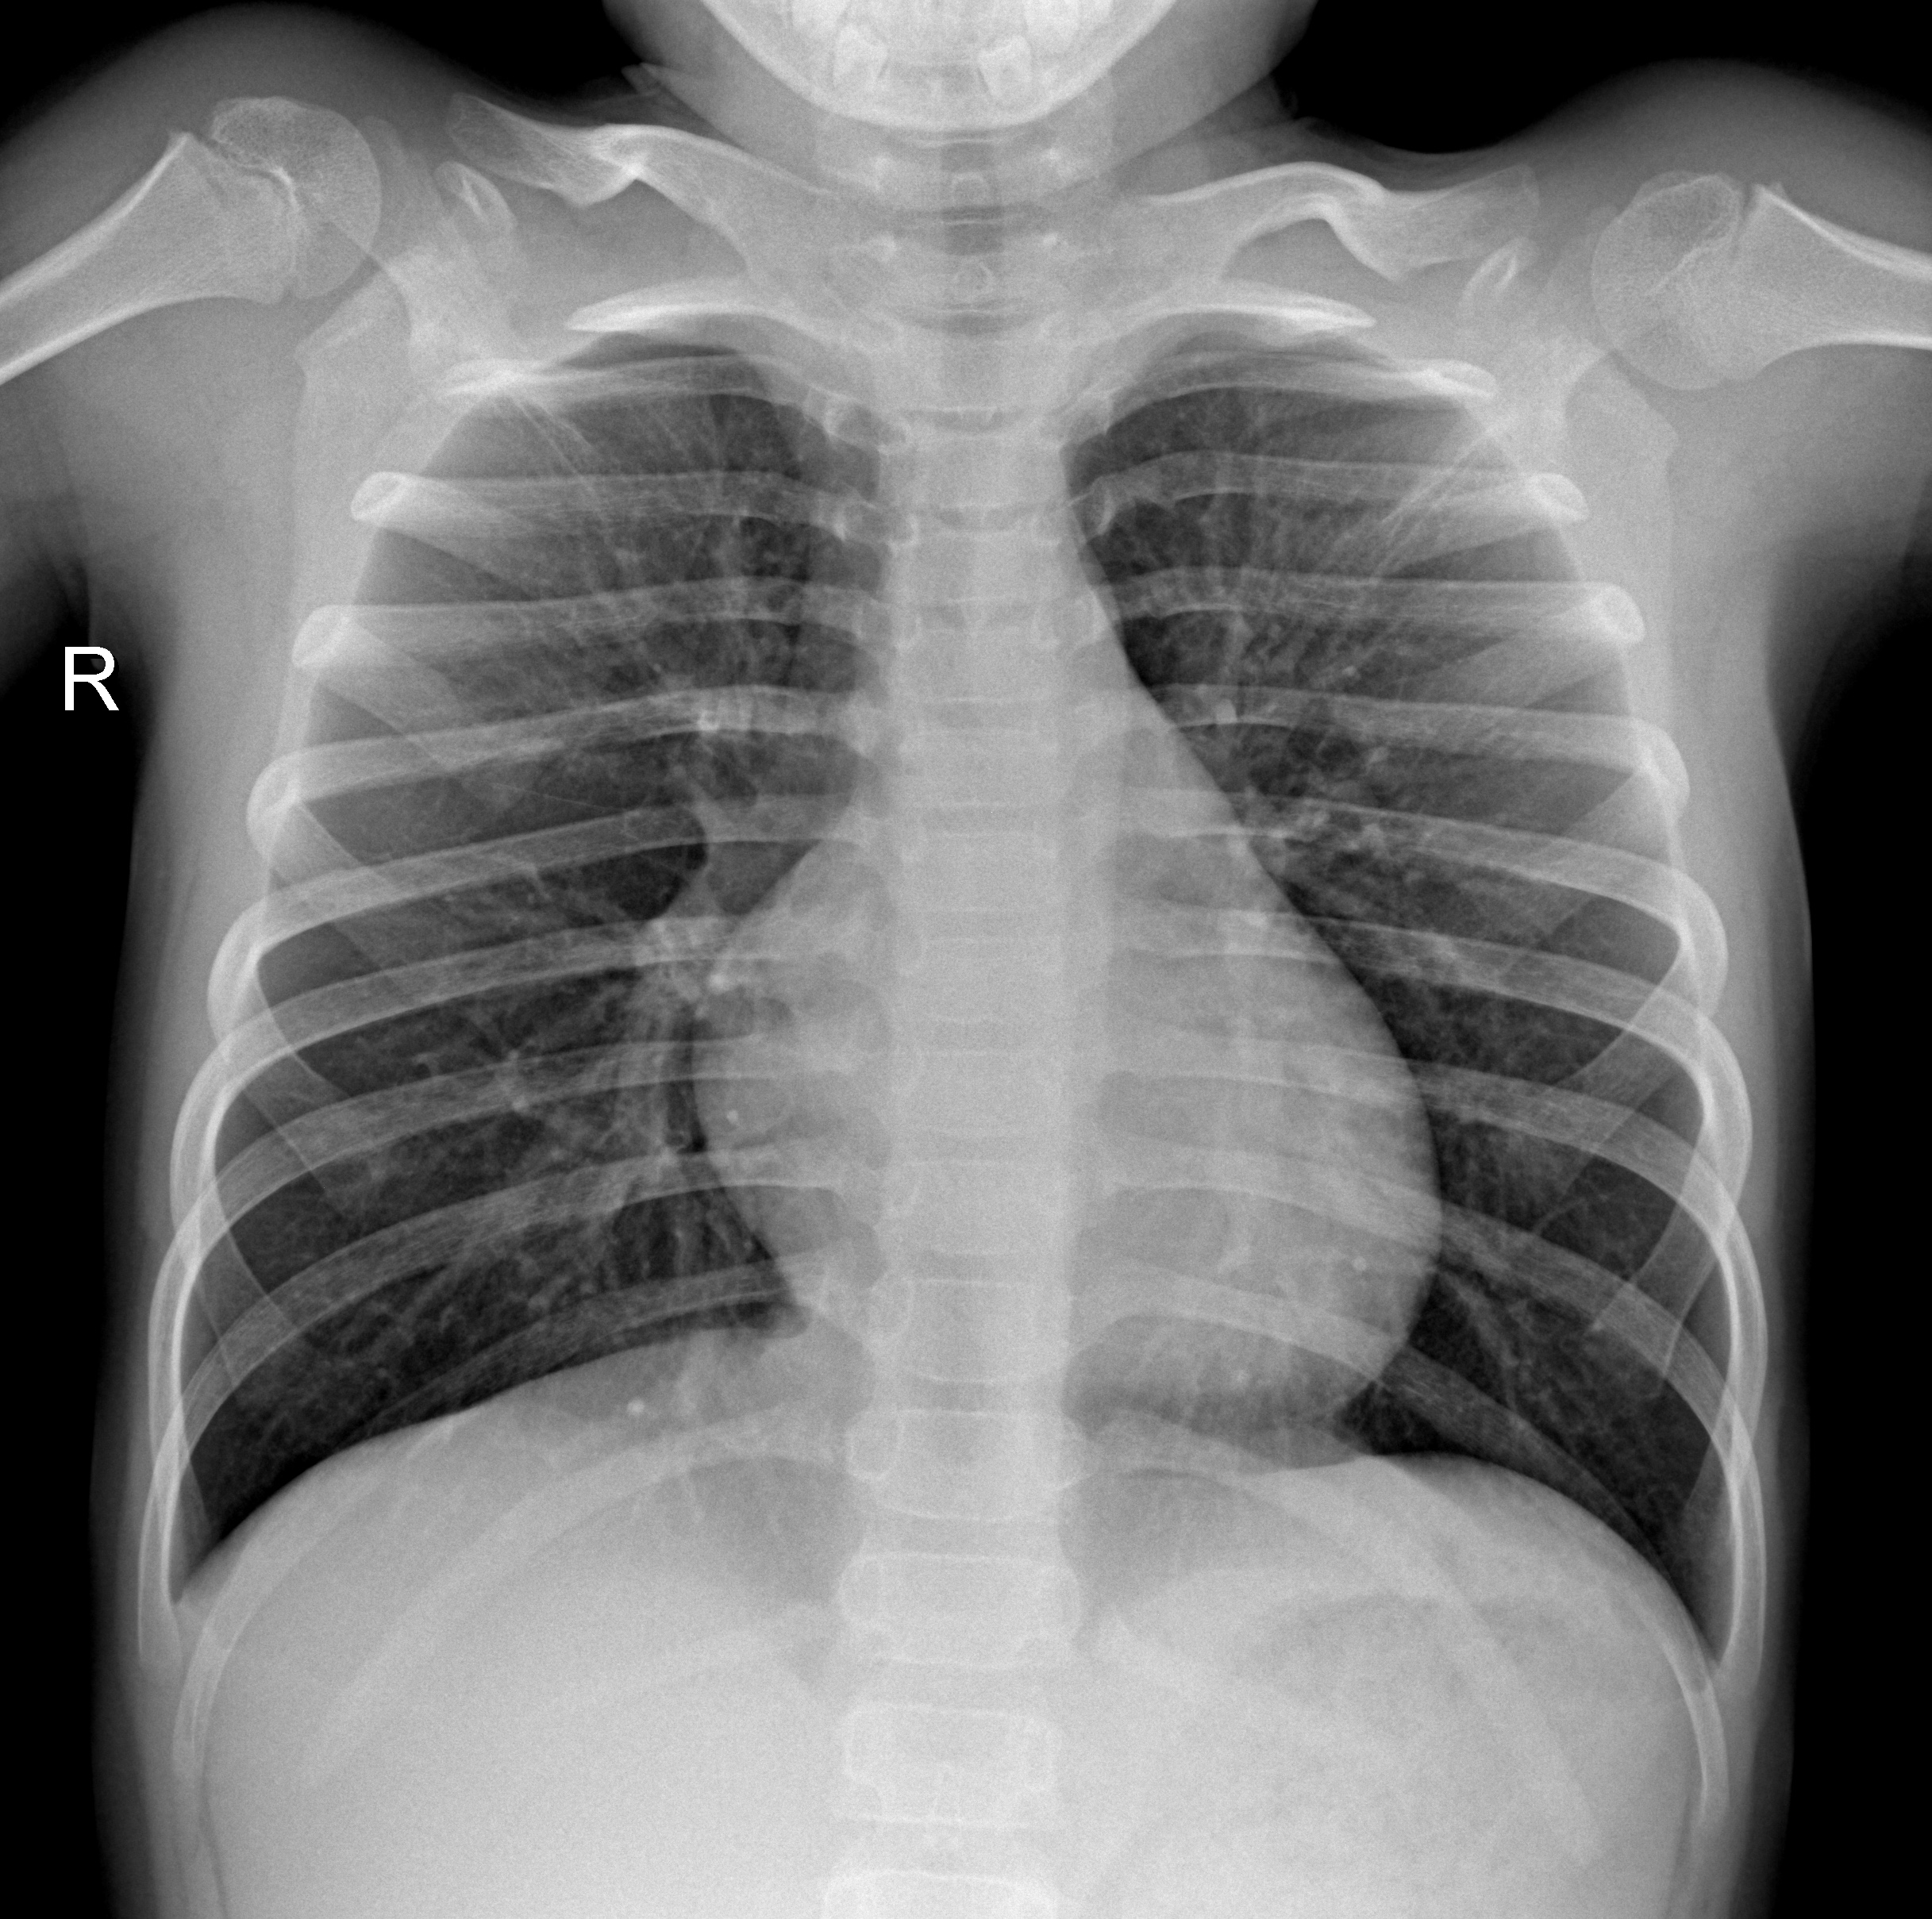
\includegraphics[width=0.4\textwidth]{Proposal/SampleNORMAL.jpeg}
    \caption{A sample image without pneumonia.\label{fig:SampleNORMAL}}
\end{figure}

\begin{figure}[H]
    \centering
    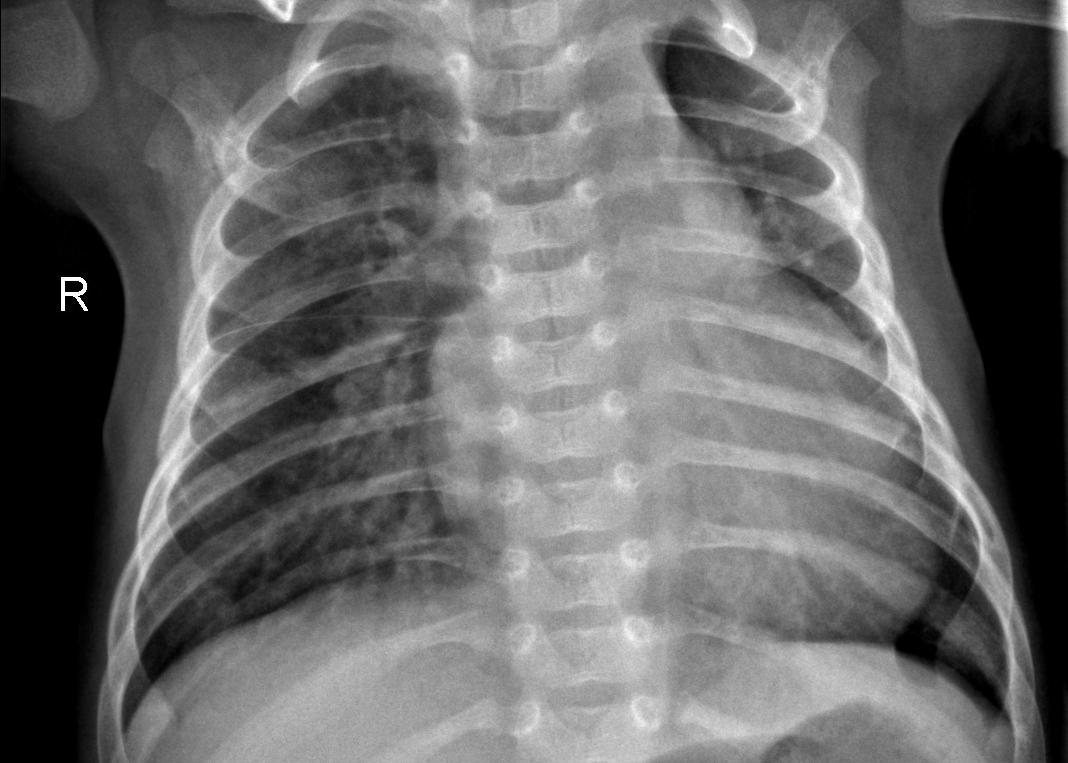
\includegraphics[width=0.5\textwidth]{Proposal/SamplePNEUMONIA.jpeg}
    \caption{A sample image with pneumonia.\label{fig:SamplePNEUMONIA}}
\end{figure}

\subsection{Potential issues}
The dataset has already been pre-emptively split into training and testing sets, which saves having to perform a manual split. 
However, the data itself is not immediately usable and will require further preprocessing before being used to train a model, namely due to the 
following issues:

\begin{itemize}
    \item Images are different resolutions.
    \begin{itemize}
        \item The sample images vary widely in resolution, with some being substantially higher than others.
        The neural network's input layer will be fixed in size, meaning all input data must be the 
        same size or the network will be unable to process it. This can be addressed programmatically using Keras to automatically resize 
        all images to a given resolution.
    \end{itemize}
    \item Class imbalance
    \begin{itemize}
        \item The training set contains 1,349 samples of patients without pneumonia, but 3,883 samples of patients with pneumonia.
        This will lead to the model favouring those with pneumonia rather than the underrepresented class of those without. This can be addressed 
        using the techniques discussed in Appendix A.
    \end{itemize}
\end{itemize}


% \begin{longtable}{ | p{0.25\textwidth} | p{0.65\textwidth} | }
%     \hline
%     \cellcolor{blue!25} Issue & \cellcolor{blue!25} Explanation \\
%     \hline
%     Images are not all the same resolution. & The neural network's input layer will be fixed in size, meaning all input data must be the 
%     same size or the network will be unable to process it. This can be addressed using Keras to automatically resize all images to a given 
%     resolution.\\
%     \hline
%     Class imbalance & The training set contains 1,349 samples of patients without pneumonia, but 3,883 samples of patients with pneumonia.
%     This will lead to the model favouring those with pneumonia rather than the underrepresented class of those without. This can be addressed 
%     using the techniques discussed in Appendix A.\\
%     \hline
%     \caption{The issues with the dataset before any preprocessing.}\label{tab:DatasetIssues}
% \end{longtable}

% ? 234 TestNorm, 390 TestPneu. 1349 TrainNorm, 3883 TrainPneu.

\pagebreak 

\section{Data science problem}
This dataset poses a clear data science problem pertaining to the binary classification of these images which will be addressed through the 
development of a convolutional neural network image classification model leveraging supervised learning. 
The ground truth is present within the dataset through its file structure\footnote{Because \textcite
{kermanyIdentifyingMedicalDiagnoses2018}'s work was not only on pneumonia, the Mendeley ZIP file contains two 
separate datasets. This proposal is only for the "chest\_xray" dataset.}, shown below:


\begin{verbatim}
    .
    `-- chest_xray/
        |-- test/
        |   |-- NORMAL/
        |   |   |-- NORMAL-4512-0001.jpeg
        |   |   |-- NORMAL-11419-0001.jpeg
        |   |   `-- ...234 more images
        |   `-- PNEUMONIA/
        |       |-- BACTERIA-40699-0001.jpeg
        |       |-- VIRUS-4190128-0001
        |       `-- ...388 more images
        `-- train/
            |-- NORMAL/
            |   |-- NORMAL-28501-0001.jpeg
            |   |-- NORMAL-32326-0001.jpeg
            |   `-- ...1347 more images
            `-- PNEUMONIA/
                |-- BACTERIA-7422-0001.jpeg
                |-- VIRUS-12220-0001.jpeg
                `-- ...3881 more images
\end{verbatim}

\noindent Files of the appropriate class are stored in the relevant subfolder\footnote{Shown file names are given as examples, and are not in the direct order they appear in the folders.}.
When this dataset is loaded, it will be possible to 
assign the relevant label to each image based on its subfolder of origin. Note that while there are separate files for bacterial and 
viral pneumonia, an analysis of other works using this dataset, seen in Chapter 2, indicated that this will not be an issue.

% "The aim is to develop a deep learning model to classify images into X classes."
% ? Describe the need for critical evaluation of the model.

% ! Footnote that the dataset contains multiple data science problems. I am only using "chest_xray", the 
% ! pneumonia identification problem.


\chapter{Related work}

% ! Added a ton of papers using this dataset to Zotero.
% ? You can use Litmaps to find more.

\section{Introduction}
This section of the report aims to demonstrate the main concepts
of related techniques that have been previously used to solve the problem 
through a thorough review of surrounding literature.

% ? What have other people done to solve it? How did they do it? 

\section{Original machine learning methods}
% ! This section was written while stressed-out and sleep-deprived and is likely absolute waffle that should be deleted.
Traditional machine learning methods such as Random Forests, K-Nearest Neighbours and Support 
Vector Machines have previously been leveraged for pneumonia classification as seen in the works of 
\textcite{ortiz-toroAutomaticDetectionPneumonia2022}. They state that leveraging these traditional approaches
alongside the creation of handcrafted textural features 'offers good performance with very low computational complexity',
as seen in their results wherein they attained an F1-Score
% ! Equation here for F1.
of 93\%.

\para However, leveraging traditional methods on detailed image datasets such as \textcite{kermanyIdentifyingMedicalDiagnoses2018}'s
relies upon manual feature engineering of textural features, which can unintentionally introduce bias. Dataset bias can significantly harm the generalisation capabilities of produced models \autocite{selvarajuGradCAMVisualExplanations2017}.
This is because it is possible that the new data given to a deployed model would differ from the preset features used on the original dataset,
which a biased model would be unable to accurately predict, unlike deep learning methods which can automatically interpret features without 
manual intervention.

% ? Wang et al. (2021) is a good paper showing the difference between traditional & deep learning results, especially Section 4.2 of it.

\section{Deep Neural Networks}
% * Neural networks themselves (Types [CNN, etc.])

% ! Find a third topic to add, though I'm not sure what it could be. 





\chapter{Proposed model}
"This section should demonstrate the suitability of
the proposed solution in solving the data science problem"

% ? The model proposed here doesn't *need* to be the one you eventually use, but you should.

% ! Add the word count to the title page before submission.

% ? When you submit your code, don't use your coloured comments like these.


\addcontentsline{toc}{chapter}{Bibliography}

% ? Prevents bibliography overflowing hbox at the expense of it taking up more lines on the page.
\emergencystretch=1em
\printbibliography

% Interesting trick to instead make the chapter number the letter A for this appendix.
\begingroup
\renewcommand\thechapter{A}
\titleformat{\chapter}[display]
{\normalfont\huge\bfseries}{}{20pt}{\Huge}
\setcounter{section}{0} % Set the section counter back to 0 so earlier chapters don't interfere.
\setcounter{figure}{0} % Set the figure counter back to 0 so earlier figures don't interfere.

\chapter*{Appendix A - Windows Subsystem for Linux}
\addcontentsline{toc}{chapter}{Appendix A - Windows Subsystem for Linux}
\markboth{Appendix A}{}

As of TensorFlow 2.10's release in September 2022, Windows is no longer natively supported with GPU access \autocite{tensorflow_install_nodate}.
To circumvent this issue, the official TensorFlow Docker container can be pulled and used on a Windows host \autocite{tensorflow_install_nodate-1}.
Docker aims to mitigate issues of software incompatibility across devices through containers, which act similarly to virtual machines 
in that they emulate another system with the necessary dependencies on a host. In this specific case, Docker uses the Windows Subsystem for 
Linux to virtualize an Ubuntu client that supports TensorFlow's latest releases with GPU support.

\para \textbf{I'm not going to remove this section until I make a final decision on the following:}
\begin{itemize}
    \item My RTX 3060 Ti seems to work at the same speed, if not slower, than a Colab GPU.
    \item My CPU works over 1000x faster than both, but my research shows that this is true for small datasets and the time needed grows exponentially.
    \item It is possible that the GPU speed issues are due to low VRAM allocation, but this cannot actually be resolved without \textbf{DUAL-BOOTING LINUX.}
    \item Though, is that even necessary? Tensorflow 2.10 is a version that supports the 3060Ti. If half of the things online use completely outdated 
    Python versions, why shouldn't I use a slightly outdated TensorFlow version?
    \item All in all, the decision between Colab and local use will depend entirely on the size of the chosen dataset, though it's likely Colab will win 
    out. 
\end{itemize} 

\end{document}